\documentclass[class=report,crop=false, 12pt]{standalone}
\usepackage[screen]{../myscratch}

\begin{document}


\titre[E]{Sons}
%===============================


\begin{enigme}[La musique du sinus]

On joue une note en fonction des décimales de $\sin( 97 \times n )$ pour  
$n=1,2,3,\ldots$

Le sinus d'un nombre est un nombre réel entre $-1$ et $+1$.
Par exemple, pour $n = 5$ 
$$\sin( 97 \times 5 ) = 0.{\color{red}81}91\ldots$$
Les deux premières décimales sont $81$, on jouera donc pour $n=5$ la note $81$ !



Pour $n$ variant de $1$ à $100$, Scratch joue la note associée aux deux premières décimales de $\sin( 97 \times n )$, avec les conditions suivantes :
\begin{enumerate}
  \item Le sinus doit être positif. (Par exemple pour $n=10$, $\sin( 97 \times 10)=-0.93\ldots< 0$ donc on ne joue aucun son.)
  \item La note doit être $>30$ (sinon le son est trop grave). (Par exemple pour $n=15$, $\sin( 97\times 15 )=0.2588\ldots$, alors \codeinline{note}\, $=25$, donc on ne joue aucun son.)
\end{enumerate}


\bigskip

\textbf{Question.} Combien de notes vont être jouées, lorsque $n$ varie de $1$ à $100$ ?


\bigskip

\emph{Indications.}
Voici une façon d'extraire les deux premières décimales :
\begin{center}
\ovaloperator{\selectmenu{plancher} de  
   \ovaloperator{\ovalnum{100} *
     \ovaloperator{\selectmenu{sin} de \ovaloperator{\ovalnum{97} * \ovalvariable{n}}}
   }
}
\end{center}

\begin{itemize}
  \item On calcule d'abord $\sin(97 \times n)$. C'est un nombre réel entre $-1$ et $+1$.
  (Pour $n=5$, $\sin(97 \times 5) = 0.8191\ldots$)
  \item On multiplie ce nombre par $100$. On obtient donc un nombre réel entre $-100$ et $+100$. (Pour $n=5$, $100 \times \sin(97 \times 5 ) = 81.91\ldots$)
  \item La fonction \codeinline{plancher} ne retient que la partie entière.
(Donc pour $n=5$, on retient \codeinline{note}\,$ = 81$.)
\end{itemize}



%\begin{solution}
%Nombre de notes jouées : $41$.
%\end{solution}

\end{enigme}



\begin{enigme}[Le sinus amorti]

Lorsque le son se propage, il peut être amorti ; c'est-à-dire que l'onde perd de l'énergie en avançant. Voici une onde amortie dessinée par Scratch :
%
%\begin{center}
%  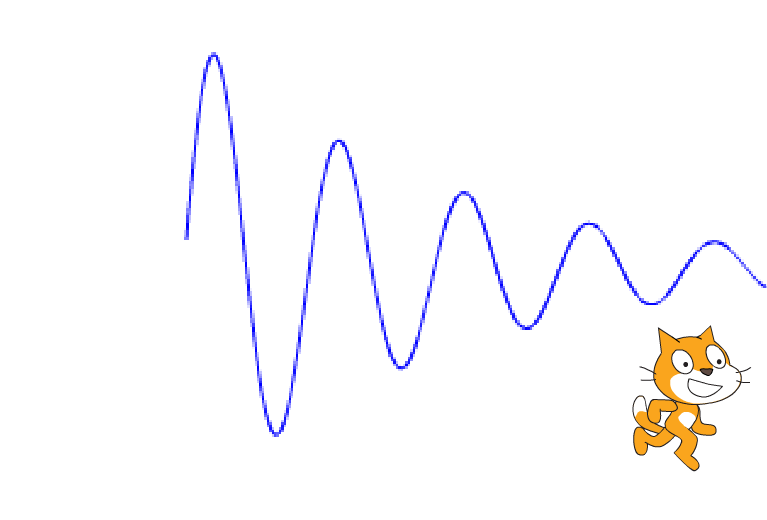
\includegraphics[scale=\scaleecran]{ecran-09-eg2} 
%\end{center}

\myfigure{0.8}{
\tikzinput{ecran-09-eg2}
}

La formule pour dessiner cette courbe est :
$$y = 100 \times e^{-0.01 \times x} \times \sin(7 \times x)$$

Dans la pratique, Scratch se déplace successivement aux points $(x,y)$ avec $0 \le x \le 240$ où $y$ est donné en fonction de $x$  par la formule :


\begin{center}
\ovaloperator{\ovalnum{100} *
  \ovaloperator{
    \ovaloperator{\selectmenu{e\^{}} de \ovaloperator{\ovalnum{-0.01} * \ovalvariable{x}}}
    *
    \ovaloperator{\selectmenu{sin} de \ovaloperator{\ovalnum{7} * \ovalvariable{x}}}
  }
}
\end{center}



\textbf{Question.} Quelle est la hauteur $y$ du second pic ? Réponds en donnant un entier, une erreur de $\pm2$ est tolérée !
\bigskip



\emph{Indications.} 
\begin{itemize}
  \item Le second pic est indiqué par la flèche sur le dessin.
  \item La hauteur du premier pic est de $88$ environ.
  \item La fonction qui permet d'obtenir cet amorti est la fonction exponentielle $e^x$ et se trouve dans la liste des fonctions mathématiques (catégorie \og{}Opérateurs \fg{}).
%  \item Afin de visualiser précisément l'endroit repéré par les coordonnées affichées, réduis la taille de Scratch au maximum et amène le à la position à étudier.
\end{itemize}


%\begin{solution}
%Réponse : 52 (donc 50, 51, 52, 53, 54 sont valides).
%\end{solution}

\end{enigme}



\begin{enigme}[La musique de Shakespeare]

L'utilisateur rentre une phrase, l'ordinateur joue une musique en fonction des caractères de la phrase.

\medskip

Voici la règle du jeu :
\begin{itemize}
  \item si la lettre est \mot{E}, la note jouée est un \emph{do} (60),
  \item si la lettre est \mot{S}, la note jouée est un \emph{ré} (62), 
  \item si la lettre est \mot{A}, la note jouée est un \emph{mi} (64),
  \item si la lettre est \mot{I}, la note jouée est un \emph{fa} (65),   
  \item si la lettre est \mot{N}, la note jouée est un \emph{sol} (67),
  \item si la lettre est \mot{T}, la note jouée est un \emph{la} (69),
  \item pour les autres caractères (y compris une espace) aucune note n'est jouée.    
\end{itemize}

\medskip

\emph{Attention, il y a une règle supplémentaire :} on joue une note pour un caractère uniquement si la lettre qui le précède dans la phrase n'est pas un \mot{E}.

\bigskip

Par exemple : \mot{MESSAGE ESSAI} va jouer les 8 notes : \emph{do ré mi do do ré mi fa.} En effet
\mot{M} ne joue pas, \mot{E} joue un \emph{do},
le premier \mot{S} n'est pas joué car la lettre précédente en un \mot{E}, par contre le second \mot{S} joue un \emph{ré}, \mot{A} joue un \emph{mi},
\mot{G} ne joue rien, \mot{E} joue un \emph{do}, l'espace entre les deux mots ne joue rien, le \mot{E} qui démarre le second mot joue un \emph{do} (le caractère précédent est une espace)...


\bigskip

Voici une phrase :
\begin{center}
\begin{minipage}{0.8\textwidth}
\center
\mot{ETRE OU NE PAS ETRE TELLE EST LA QUESTION C EST SHAKESPEARE QUI LE DIT DANS HAMLET}
\end{minipage}
\end{center}


\textbf{Question.} Combien de notes vont être jouées ?

\bigskip

\emph{Indications.}
\begin{itemize}
  \item Afin de permettre à Scratch de jouer des sons, ajoute l'extension \og{}Musique\fg{}.
  \item Fais attention à ne pas faire de faute en recopiant la phrase. %Copie-colle la phrase pour éviter les erreurs de frappe.
  \item Ajoute un temps aléatoire pour la durée de chaque note afin d'avoir une musique moins monotone.
\end{itemize}

%\begin{solution}
%Réponse : 34 notes.
%\end{solution}

\end{enigme}


\end{document}

